\section{Experiments}
\label{sec:experiments}

We discuss the benefits and drawbacks of our framework in this section.
In the first place, parameters choosing and tuning are important issues in decolorization.
Experienced users can use proprietary programs such as Adobe Photoshop 
to create their desired grayscale images.
However, such editing is not familiar to amateurs, so an automatic algorithm seeking 
a solution to facilitate this process without users' interference is necessary.
On the other hand, performance is also an important issue. 
Users expect outputs immediately because the baseline algorithm, eg. rgb2gray, 
is really fast to perform the color conversion.
A competitive algorithm should not far from this performance unless it deals with
particular details and makes tremendous different results.
Our algorithm has benefits on tuning parameters and compatible performance.
Moreover, our algorithm maintain the visual appearance in general unless the limited
cases which would be discussed in the end of this section.

\begin{figure}[t]
\begin{center}
\begin{tabular}{ccc}
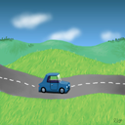
\includegraphics[width=0.27\linewidth]{fig/Voiture.png} &
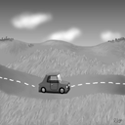
\includegraphics[width=0.27\linewidth]{fig/Voiture-sparse_dr-colorT03_resize01.png} &
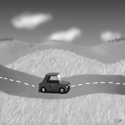
\includegraphics[width=0.27\linewidth]{fig/Voiture-sparse_dr-colorT02_resize01.png} \\
%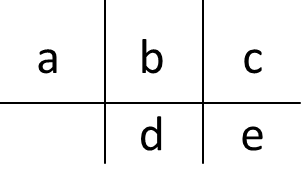
\includegraphics[width=0.10\linewidth]{fig/abcde.png} &

\includegraphics[width=0.27\linewidth]{fig/Voiture-visD-all.png} &

\includegraphics[width=0.27\linewidth]{fig/Voiture-visD-colorT03.png} & 

\includegraphics[width=0.27\linewidth]{fig/Voiture-visD-colorT02.png} \\
\end{tabular}
\caption{
\textbf{Effect of the threshold by choosing different atoms.} 
From left to right, up to down with alphabet order:
(a) original image,
(b) ours with $\delta=0.3$,
(c) ours with $\delta=0.2$,
(d) mean color from the segmentation of original image in saliency descent order,
(e) dictionary with $\delta=0.3$,
(f) dictionary with $\delta=0.2$.
Our algorithm picks atoms follow in saliency descent order. In this case, comparing with
Olive Drab (the third atom of (d)), Sea Green (the forth atom of (e)) is too similar 
under the threshold $\delta=0.3$,
so our algorithm choose Sky Blue under this setting.
When Sea Green is considered as basis, the difference between two similar colors
will be amplified.}
\label{fig:parameters}
\end{center}
\end{figure}

\subsection{Parameters}
\label{sec:parameters}
The main problem of decolorization is complicated parameter setting.
Most of the algorithms need to decide lots of parameters because 
their operators inherently have more complicated function.
For instance, the offset angle of color wheel serves the task of preventing
saliency lost in~\cite{Gooch:2005:CSC,Ancuti:2011:ESG}.
It controls the mapping between chromatic and illuminance differences.
By assigning particular angle, the operators could enhance detail for
color-deficient observers.
While to embedded these kind of parameters in algorithm risk to make unwanted artifact.
In contrast with these methods, we avoid to introduce offset angle and 
utilize some preliminary information to prevent the saliency lost.

Our framework, combining segmentation, saliency map computation, and dimensionality
reduction by sparse model, seems complicated at first glance,
but these factors can be friendly applied with their default setting for most of cases
in our experiments.
The main point in our framework is to construct the dictionary $D$,
and the chief parameter behind this procedure is the color threshold $\delta$.
Our procedure decides whether a color is suitable for adding in the dictionary by
judging if this color exceeds the colors have been collected over the threshold $\delta$.
In our experiment, this factor is reliable only if we have special requirement
to distinguish similar color in grayscale.
Figure~\ref{fig:parameters} illustrates the function of this parameter.
Without notification, we use the default parameter $\delta=0.3$ for all results in
this paper.

%

\begin{figure}[t]
\begin{center}
\begin{tabular}{cccc}
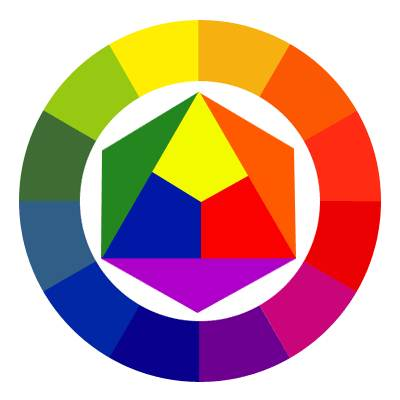
\includegraphics[width=0.2\linewidth]{fig/colorwheel.jpg} &
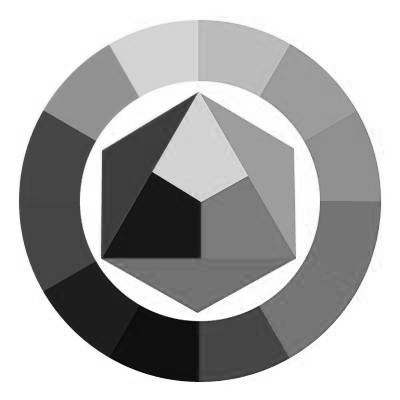
\includegraphics[width=0.2\linewidth]{fig/colorwheel-sparse_dr.png} &
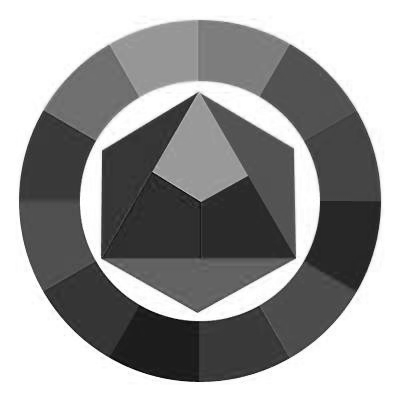
\includegraphics[width=0.2\linewidth]{fig/colorwheel-pca_rgb.png} & 
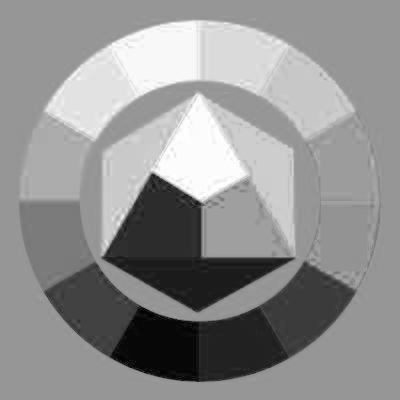
\includegraphics[width=0.2\linewidth]{fig/colorwheel-pca_lab.png} \\
color & ours & RGB & CIE{\it L*a*b}
\end{tabular}
\caption{
\textbf{Dimensionality reduction on difference spaces.}
The comparison between our method and PCA directly applying on RGB and CIE{\it L*a*b}
demonstrates the sensitivity of PCA on different basis. Our method chooses a reasonable
basis for individual input images.
}\label{fig:PCA}
\end{center}
\end{figure}



\begin{figure}[t]
\begin{center}
\begin{tabular}{ccc}
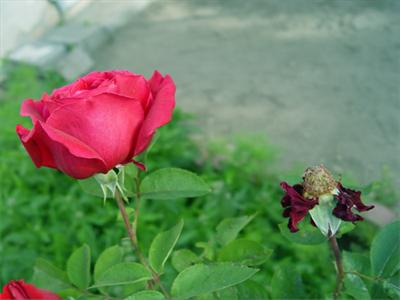
\includegraphics[width=0.3\linewidth]{fig/2_75_75169.png} &
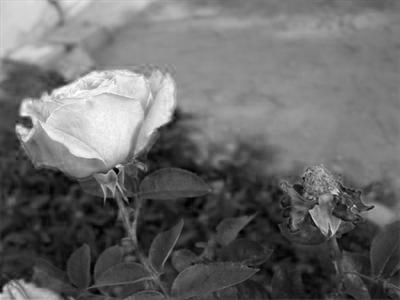
\includegraphics[width=0.3\linewidth]{fig/2_75_75169-sparse_dr.png} & 
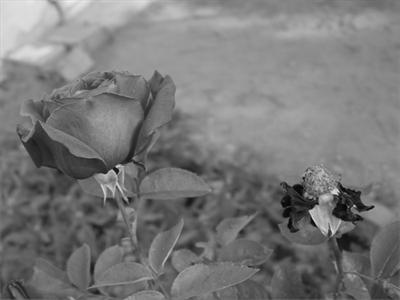
\includegraphics[width=0.3\linewidth]{fig/2_75_75169-rgb2gray.png} \\
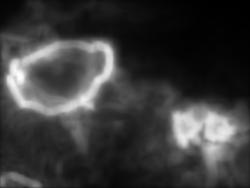
\includegraphics[width=0.3\linewidth]{fig/2_75_75169_SaliencyMap.jpg} &
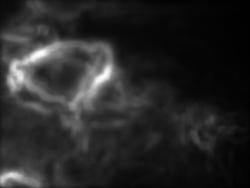
\includegraphics[width=0.3\linewidth]{fig/2_75_75169-sparse_dr_SaliencyMap.jpg} & 
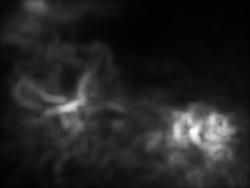
\includegraphics[width=0.3\linewidth]{fig/2_75_75169-rgb2gray_SaliencyMap.jpg} \\
color & ours & rgb2gray \\
\end{tabular}
\caption{
\textbf{Saliency preserving decolorization.}
The first row shows the original color image and three different grayscale images,
and the second row shows the saliency detected by~\protect\cite{Hou:2012:ISH} 
on them. When an unavoidable information loss occurs,
our method prior preserves the saliency on significant regions in grayscale.
In this case, there are two followers in the image, the left one was chose by
purposed algorithm.
}\label{fig:saliency}
\end{center}
\end{figure}

\subsection{Salient object preserving}
\label{sec:saliency}
Our method can be viewed as performing PCA on higher dimensional space
rather than the original color space.
While PCA has been studied for decolorization in~\cite{Gooch:2005:CSC}, the space
of applying such technique was vague and it is worth to discuss herein.
As discussion in~\cite{Gooch:2005:CSC}, PCA is quite sensitive in which computation
takes place. Figure~\ref{fig:PCA} shows that performing PCA on color spaces such as
RGB and CIE{\it L*a*b} have dramatic differences.

The point is our framework effectively chooses specific color codewords, namely basis,
to perform PCA, and the data on the basis reveal a good structure for preserving saliency
after applying dimensionality reduction.
We discuss the property by analyzing the scatter matrix of the data points
and applying saliency detection after decolorzing on these two spaces.

To tell the difference between original color space and the hyperspace,
we first explore the ratio of the largest eigen value $\lambda_1$ over 
the sum of all eigen value on the scatter matrix of the pixels sample from a space, 
denote the ratio by 
$r = \lambda_1 / \sum_i \lambda_i$.
Theoretically, data are easier to be represented in single channel 
by dimensionality reduction with higher $r$. 
We computed the ratio over $24$ color images in the collection of~\cite{Ancuti:2011:ESG}.
The mean of $r$ is equal to $0.8491$ and $0.8169$ on the hyperspace and the original color
space, so the difference is not distinguish at first sight.
However, the salient regions in grayscale 
have obviously different distribution on the two spaces.
Figure~\ref{fig:saliency} demonstrate this observation.
Our algorithm visually preserves the salient region as the original image.
Moreover, we apply saliency detection algorithm on color and grayscale images, and
the results make the differences more definite.

\newcommand{\sfont}{\scriptsize}
\newcommand{\rb}[1]{\raisebox{1.0ex}[0pt]{#1}}
\begin{table}[t]{\tiny
\caption{\textbf{The computation time of a $710\times480$ input image.}} 
\begin{center}{\sfont
\begin{tabular}{|>{\centering}p{1cm}|>{\centering}p{1cm}|>{\centering}p{1cm}|>{\centering}p{1cm}|>{\centering}p{1cm}|>{\centering}p{1.1cm}|p{1cm}<{\centering}|} \hline%
              &             &               &              &              &                  &          \\%
\rb{Method}   &  \rb{Ours}  & \rb{Ancuti11} & \rb{Kim09}   & \rb{Smith08} & \rb{Grundland07} &  \rb{Gooch05} \\ \hline %
              &             &               &              &              &                  &          \\%
\rb{Running}  &  \rb{1 sec} & \rb{1 sec}    & \rb{0.5 sec} & \rb{11 sec}  & \rb{0.1 sec}     &  \rb{5 min}   \\ \hline %
\end{tabular}}
\end{center}
\label{tbl:performance}}
\end{table}

\subsection{Performance}
\label{sec:performance}
The results were generated by a non-optimized MatLab code on a Personal Computer 
with four-core Intel CPU and 16 GB RAM.
The computational time of our algorithm is dominated by solving the lasso problem.
While this step only play the rule of checking the dictionary rank, in other words,
we do not need to solve it for total amounts of the input pixels.
We downsample the image for speeding up the whole procedure.
The performance raise ten times from $10$ to $1$ second on a $710\times480$ image by
reducing the input image to $71\times48$ under our implementation.
By our experiment, sampling on the thumbnail image with approximate thousand of pixels
is enough to present results in our paper.
Table~\ref{tbl:performance} lists the computation time for reference.
To speed up current implementation, parallel computation on lasso and random sampling
of rotation matrix is available without modified the framework.
Other advance approaches such as lasso screening~\cite{Xiang:2011:LSP} are also
encouraged to reduce the computation complexity. 
Since our method performs on the dictionary constructed by superpixels, 
it has very limited memory requirement comparing with 
the pixel-based methods~\cite{Gooch:2005:CSC}.
The typical dictionary size is from $5$ to $7$, depend on the color distribution of 
input image.
Because the size of dictionary is not proportion to image size, 
our method is suitable to scale up for high resolution image.
